\chapter*{Introduction: A New Language for Thinking About Thinking Machines}
\label{chap:introduction}
\addcontentsline{toc}{chapter}{Introduction: A New Language for Thinking About Thinking Machines}

\begin{figure}[h]
    \centering
    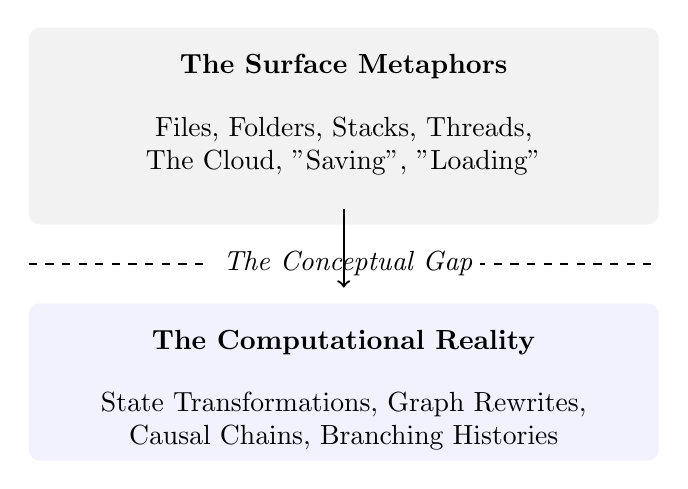
\begin{tikzpicture}
        % Surface Level
        \fill[gray!10, rounded corners] (-4, 2) rectangle (4, 4.5);
        \node at (0, 4) {\textbf{The Surface Metaphors}};
        \node[align=center] at (0, 3) {Files, Folders, Stacks, Threads, \\ The Cloud, "Saving", "Loading"};
        
        % The Barrier
        \draw[thick, dashed] (-4, 1.5) -- (4, 1.5);
        \node[fill=white, inner sep=2pt] at (0, 1.5) {\textit{ The Conceptual Gap }};
        
        % The Reality
        \fill[blue!5, rounded corners] (-4, -1) rectangle (4, 1);
        \node at (0, 0.5) {\textbf{The Computational Reality}};
        \node[align=center] at (0, -0.5) {State Transformations, Graph Rewrites, \\ Causal Chains, Branching Histories};
        
        % Connection
        \draw[->, thick] (0, 2.2) -- (0, 1.2);
    \end{tikzpicture}
    \caption{The disconnect between the language we use to describe computers and the reality of how they operate.}
    \label{fig:surface_vs_reality}
\end{figure}

Computers are nowhere near as simple as we pretend.

We cling to metaphors inherited from the early days of computing, relics of the 1970s and 80s that have calcified into dogma. We speak of files, processes, threads, stacks, heaps, and the ethereal "cloud." We visualize our data as documents sitting in folders, or as distinct objects interacting in a rigid hierarchy. These familiar terms offer a comforting, if superficial, surface view of the digital world—a user interface for the mind. Yet, lurking beneath this established lexicon lies an operational reality that is far stranger, infinitely deeper, and universally consistent: a fundamental world constructed entirely from \textbf{transformations}.

The entire digital cosmos is built on change. There is no such thing as static data; there is only data waiting to be rewritten.

Every line of code, every massive distributed system, every intricate relational database, every photo-realistic simulation, every nuanced AI model, every frustrating bug report, and every massive scientific computation—all of it—is ultimately an emergent phenomenon. It is built from atomic rules acting upon structured data, progressing step by deliberate step, from one defined state to the next. It is a perpetual chain of cause, effect, and mutation.

Despite erecting the entire edifice of modern civilization upon this dynamic, computational substrate, our ability to reason about it remains strikingly deficient. We lack a sophisticated, agreed-upon vocabulary for describing the \textbf{shape of computation}. We are conceptually impoverished, unable to adequately articulate how programs truly evolve, how state transforms over time, how alternative possibilities interrelate, how execution histories converge or diverge, and how different, co-existing "universes" of behavior can reside within even the most rudimentary system. 

In physics, we have a language for how matter moves through space and time. In computing, we generally only have a language for the instructions we give the machine, not for the behavior that emerges from them. In essence, we lack a \textbf{physics of computation}.

This book is a determined effort to construct that essential vocabulary, to forge a language capable of mapping the computational cosmos.

\section{Why This Book Exists}
\label{sec:why-exists}

I did not write this book because I claim to have stumbled upon a fundamental, undisputable law of reality. I am not a prophet, and this is not a revelation. Instead, this endeavor is the direct result of two decades spent as a systems engineer, locked in a perpetual struggle with the overwhelming complexity of real-world software. 

My career has taken me through the trenches of cutting-edge AAA game studios, where performance is measured in microseconds; to mobile games studios managing massive concurrency; to nimble startups pivoting daily; and deep into large-scale open-source projects. Across all these diverse environments—working on gameplay logic, core engine technology, DevOps pipelines, live-ops telemetry, and business intelligence—I have seen the same chaos repeated. Whether in rigid waterfall structures or chaotic agile sprints, in disorganized organizations or meticulously planned architectures, I encountered an unyielding, consistent pattern: the tools and concepts we use to describe software are \textbf{radically weaker} than the sophisticated tools we use to build it.

Consider the prevailing descriptive frameworks we rely upon. Version control systems like Git give us a strictly linear history of a project, a sequence of commits that implies a straight line of progress. Yet, this view remains blind to the vast, branching space of what \textit{could} have happened—the potential evolution, the discarded experiments, and the structural merges that define the actual topology of code. A debugger exposes a single, narrow execution trace, effectively performing an autopsy on a frozen moment in time, but it cannot illuminate the alternative worldlines and near-misses that almost defined the outcome.

Our type systems elegantly define static structure, ensuring that shapes fit into holes, but they fail to capture the dynamic, living rewrites that breathe function and purpose into that structure. Graph theory offers the bare bones of nodes and edges, omitting the critical element of governing rules that dictate how those nodes change. Even physics provides powerful equations of motion for the natural world, but offers no semantic insight into the nature of code.

This inadequacy is becoming an existential problem. We are no longer writing scripts to sort lists. Modern AI systems—Large Language Models (LLMs), autonomous agents, and complex reasoning engines—are beginning to operate in conceptual spaces that are even more opaque and less formally describable than traditional code. We are building machines we cannot fully explain with languages that were designed to describe card sorters.

Therefore, this entire work proceeds from one clear, simple, and driving question:

\begin{quote}
    What if we had a unified, comprehensive way to think about computation—encompassing structure, change, history, and possibility—all at once?
\end{quote}

This is not offered as a simple analogy. It is not a casual metaphor to help juniors visualize pointers. It is not speculative hype. It is presented as a working, implementable model for understanding the mechanics of the digital world.

\section{What This Book Is Not}
\label{sec:what-is-not}

To be clear about its scope and ambition, this is emphatically \textbf{not a manifesto}. I am not claiming to have derived the ultimate truth of the universe, nor is this a replacement for established fields like physics, mathematics, or computer science. You will not find a new religion here, nor a "Grand Unified Theory" that claims to solve P vs NP or explain consciousness.

Instead, this book is designed to be a pragmatic toolset for the builder and the thinker. It functions as a rigorous framework for modeling state transformation, providing a conceptual lens through which to view system dynamics. It offers a powerful methodology for organizing thinking about complexity and causality, and provides a practical architecture for building verifiable, understandable systems. It is a narrative that seeks to successfully tie together previously siloed ideas from computer science, logic, and mathematics.

It represents a \textbf{computational cosmology}, but only in the most functional sense: it seeks to unify many distinct, practical views of computation under one coherent, structural roof.

\section{What This Book Is: The C\texorpdfstring{\boldmath$\Omega$}{Omega}MPUTER Model}
\label{sec:what-is}

The core model, which we call \textbf{C\texorpdfstring{\boldmath$\Omega$}{Omega}MPUTER}, represents a shift from imperative instruction to structural evolution. It is a robust system built from just three simple, yet deeply expressive, primitives.

\begin{figure}[h]
    \centering
    \begin{tikzpicture}[node distance=2.5cm]
        \node (RMG) [draw, circle, align=center, minimum size=2.5cm] {\textbf{RMG} \\ (Structure)};
        \node (DPO) [draw, circle, align=center, minimum size=2.5cm, right of=RMG, xshift=2cm] {\textbf{DPO} \\ (Laws)};
        \node (Worldline) [draw, circle, align=center, minimum size=2.5cm, below of=RMG, xshift=2.25cm] {\textbf{Worldlines} \\ (History)};
        
        \draw[->, thick, bend left] (RMG) to node[above] {Governed by} (DPO);
        \draw[->, thick, bend left] (DPO) to node[right] {Generates} (Worldline);
        \draw[->, thick, bend left] (Worldline) to node[left] {Records} (RMG);
        
        \node[align=center, below=0.5cm of Worldline] {The Trinity of \COMPUTER{}};
    \end{tikzpicture}
    \caption{The three primitives interact cyclically: Structure defines the state, Laws define the change, and History captures the path.}
    \label{fig:computer_trinity}
\end{figure}

\begin{enumerate}
    \item \textbf{Graphs within Graphs (RMGs)}: The foundational structure is provided by \textbf{Recursive Meta-Graphs}. Unlike standard flat graphs, RMGs possess the fractal ability to contain other graphs within their nodes and edges. This allows for the natural, hierarchical representation of any structured data, capable of zooming from the microscopic detail of an abstract syntax tree out to the macroscopic architecture of an entire distributed system without changing the data model.
    
    \item \textbf{Rules that Rewrite (DPO)}: The dynamic element is the application of Rules that Rewrite those Graphs, specifically utilizing the rigorous formalism of \textbf{Double-Pushout (DPO) rewriting}. If the RMG is the "matter" of our universe, DPO provides the "physics." These rules are the equations of motion for computational state, defining exactly how one graph transitions to another while preserving invariants.
    
    \item \textbf{Histories of Rewrites (Worldlines)}: The element of time and possibility is captured by the Histories of those Rewrites. We do not simply overwrite data; we trace the execution \textbf{worldlines} that detail complete provenance. This allows us to simultaneously map the path we took and the landscape of alternative possibilities we declined.
\end{enumerate}

From the combination of these three simple ingredients, a surprising and powerful amount of structural insight naturally emerges. Execution is no longer a black box, but a precise, traceable path through a vast state space. We can begin to see \textbf{Alternative Executions} not as errors, but as nearby paths that were almost taken, existing in a halo of possibility around our program. \textbf{Optimizations} are re-framed not as hacks, but as geometric shortcuts—finding different, more efficient routes to the identical destination.

Concepts that once felt distinct begin to merge. \textbf{Concurrency} is modeled simply as safe, overlapping transformations in the graph. \textbf{Bugs} cease to be ghosts in the machine and become divergent, undesired trajectories in the execution history. \textbf{Debugging} transforms from guesswork into the act of precisely comparing worldlines to find the exact coordinate where the divergence began. Even \textbf{Security Analysis} is redefined, becoming the systematic exploration of adversarial transforms—searching the graph for paths that lead to forbidden states.

None of the mechanisms described in this book are based on magic or hand-waving. All of it is computable, formal, and implementable today. This book is not about "discovering reality" in a metaphysical sense; it is about giving the builders of the future demonstrably better tools to understand and navigate the realities they create.

\section{Who This Book Is For}
\label{sec:who-for}

This book is dedicated to the diverse community of creators who recognize the limitations of our inherited abstractions. 

It is written for the \textbf{Software Engineers} who feel genuinely constrained by the computational metaphors of the past and are seeking a more robust foundational model. It is for the \textbf{Systems Thinkers} looking for a truly unified mental model that bridges the gap between static structure, logical rules, and dynamic execution. It is for the \textbf{Researchers} exploring the deep utility and expressive power of graph rewrite systems, and for the \textbf{AI Developers} wrestling with the fundamental frustration of opaque reasoning and decision-making in large probabilistic models.

But it extends beyond pure code. It is for the specialists—the \textbf{Simulation Designers}, \textbf{Game Engine Architects}, and \textbf{Distributed Systems Engineers}—who deal daily with complex state evolution and need a language to describe it. It is for the creators of devtools, compilers, runtimes, and languages who build the very foundations of the digital world. And, fundamentally, it is for anyone who senses that the concept of "computation" is far grander, stranger, and more expansive than our standard textbooks allow.

It is also for those who simply appreciate the elegance of big ideas, the strangeness of deep concepts, and the satisfaction of beautifully structured thought.

\section{Why I Had to Write It}
\label{sec:why-had-to-write}

The simple truth is: I couldn't not write it.

After years spent building and designing high-stakes systems—game engines that manage millions of objects, distributed systems requiring deterministic consensus, AI agents, provenance systems, and graph-based architectures—I observed the same few patterns emerge, time and time again. Whether I was optimizing a physics collider or debugging a race condition in a cloud service, the solution always looked the same.

\textbf{Everything is rewrite. Everything is transformation. Everything is history. Everything is structure.}

I wanted—I needed—a coherent, singular way to hold all these aspects of computation in my mind at once. I needed a way to stop seeing code as text and start seeing it as geometry.

This book is my most sincere attempt to construct that tool. It is a tool for myself first, to bring order to the chaos of my own work. It is a tool for other builders second. And, finally, it is a tool for anyone whose curiosity is piqued by the fundamental shape of computation.

Whether the ideas presented here stand the ultimate test of time is secondary to the immediate goal. The primary point is exploration. The point is possibility. The point is creating something cool, something interesting, something joyful—something that makes deep complexity feel genuinely navigable instead of permanently overwhelming.

This is my exploration.

\textbf{Welcome to C\texorpdfstring{\boldmath$\Omega$}{Omega}MPUTER.}